% !Mode:: "TeX:UTF-8:Main"
\documentclass{beamer}

\usepackage{tikz}
\usepackage{tikzlings-koalas}
\usepackage{fontspec}
\usetikzlibrary{shapes,arrows.meta}
\newfontfamily\notoemoji{Noto Color Emoji}[Renderer=HarfBuzz]

\setbeamertemplate{background canvas}{
  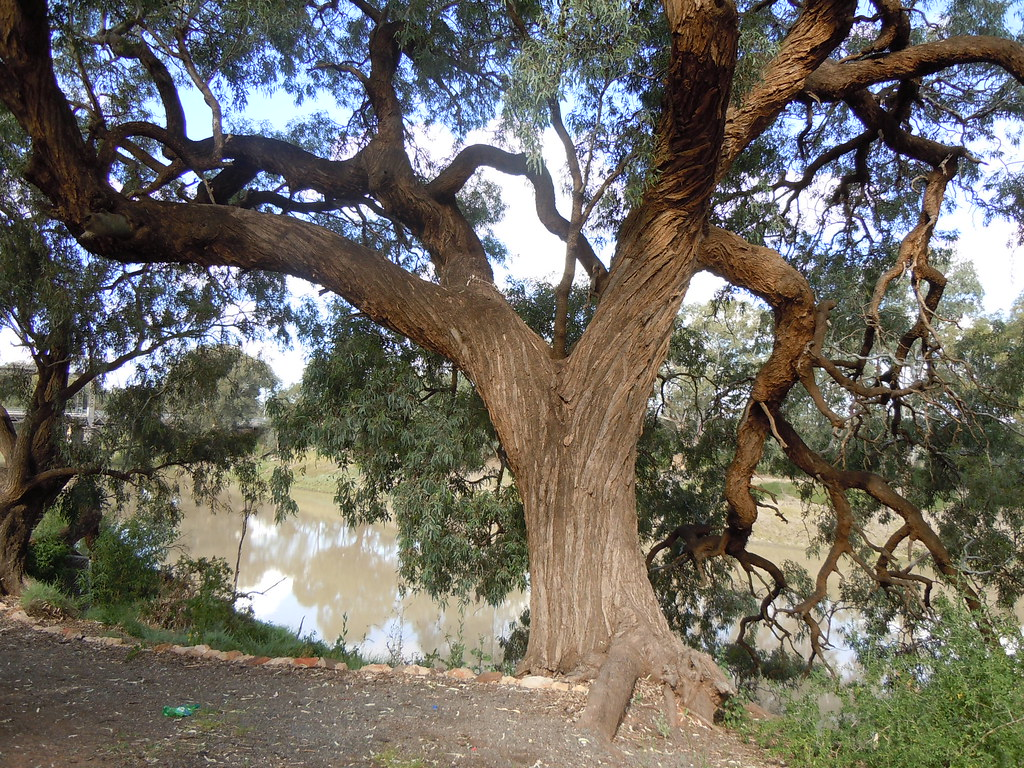
\includegraphics[height=\paperheight]{eukalyptus}
}
\setbeamertemplate{navigation symbols}{}

\begin{document}
\makeatletter\def\thing@strawhat{brown}
\newcommand\koalahookbody{\node[yshift={1cm},font=\fontsize{30pt}{30pt}\selectfont]{\notoemoji 🎸};}
\tikzset{cork/.style={brown,thick,{-Kite[]}}}
\begin{frame}

\vspace*{5.5cm}
\mbox{}\hfill
  \begin{tikzpicture}[scale=1.5,transform shape]
  \begin{scope}[rotate=10]
  \koala[shift={(0,0.3)}]
  \begin{scope}[overlay]
  \begin{scope}[xshift=-18,rotate=12,yshift=-1.1,scale=1.2]
  \fill[\thing@strawhat,rotate=-15] (0.44,2.0) ellipse[x radius=0.75, y radius=0.1];
  \fill[\thing@strawhat,rotate=-15] (0.1,2.05) rectangle (0.78,2.5);
  \fill[\thing@strawhat,rotate=-15] (0.44,2.5) ellipse[x radius=0.34, y radius=0.08];
  \fill[\thing@strawhat,rotate=-15] (-0.3,2.02) -- (1.18,2.02) -- (0.78,2.2) -- (0.1,2.2) -- cycle;
  \fill[brown!50!black,rotate=-15] (0.44,2.2) ellipse[x radius=0.34, y radius=0.08];
  \fill[brown!50!black,rotate=-15] (0.1,2.2) rectangle (0.78,2.3);
  \fill[\thing@strawhat,rotate=-15] (0.44,2.3) ellipse[x radius=0.34, y radius=0.08];
  %\draw[red,rotate=-15] (0.44,2.0) ellipse[x radius=0.75, y radius=0.1];
  \path[rotate=-15] (0.44,2.0) --++ (0.75,0)
    coordinate[pos=0](a1){}
    coordinate[pos=0.33](a2){}
    coordinate[pos=0.45](a3){}
    coordinate[pos=0.7](a4){}
    coordinate[pos=0.87](a5){}
     (0.44,2.0) --++ (-0.75,0)
    coordinate[pos=0](b1){}
    coordinate[pos=0.22](b2){}
    coordinate[pos=0.5](b3){}
    coordinate[pos=0.68](b4){}
    coordinate[pos=1](b5){};
   
  \node at (1,2.2){\tiny\notoemoji🦘};
  \end{scope}
  %\draw[red,->](a1)--++(0,-1);
  \draw[cork](a2)--++(0,-0.3);
  \draw[cork](a3)--++(0,-0.45);
  \draw[cork](a4)--++(0,-0.46);
  \draw[cork](a5)--++(0,-.4); %rechts ausßen
  %\draw[green,->](b1)--++(0,-1);
  %\draw[red,->](b2)--++(0,-0.42);
  \draw[cork](b3)--++(0,-0.35);
  \draw[cork](b4)--++(0,-0.41);
  \draw[cork](b5)--++(0,-0.42);
  
   
  \end{scope}
  \end{scope}
  \end{tikzpicture}\hspace*{3cm}
  	
\end{frame}	

\end{document}


